\section{Quantum GIS 1.0}
\pagenumbering{arabic}
\setcounter{page}{1}

Quantum GIS (QGIS) is a user friendly Geographic Information System (GIS) and
an official project of the Open Source Geospatial Foundation (OSGeo). QGIS is
written in C++ and Python with a QT based GUI. It is licensed inder the GNU
General Public License (GPL).

\minisec{History}

QGIS began life in February of 2002, with the first release in June of the
same year. The initial goal was to create a viewer for PostGIS data that ran
on GNU/Linux. From those humble beginnings, QGIS has become a true
cross-platform application that runs on all major versions of unix,
GNU/Linux, as well as Mac OS and MS Windows. It supports numerous vector,
raster, and database formats and provides a wide variety of core and external
geoprocessing functionalities.

\subsection{QGIS Open Source Community}

The QGIS project is Open Source and carried out largely by a group of
developers, translators, documenters, release helpers, bug reporters, and
promoters. All these volunteers together with a large number of users make up
the QGIS comunity, which in time has built up a comprehensive, valuable and
useful code and documentation base free to use and improve for everybody.

\begin{figure}[h]
   \begin{center}
   \caption{QGIS Community Map}\label{fig:community-map}\smallskip
   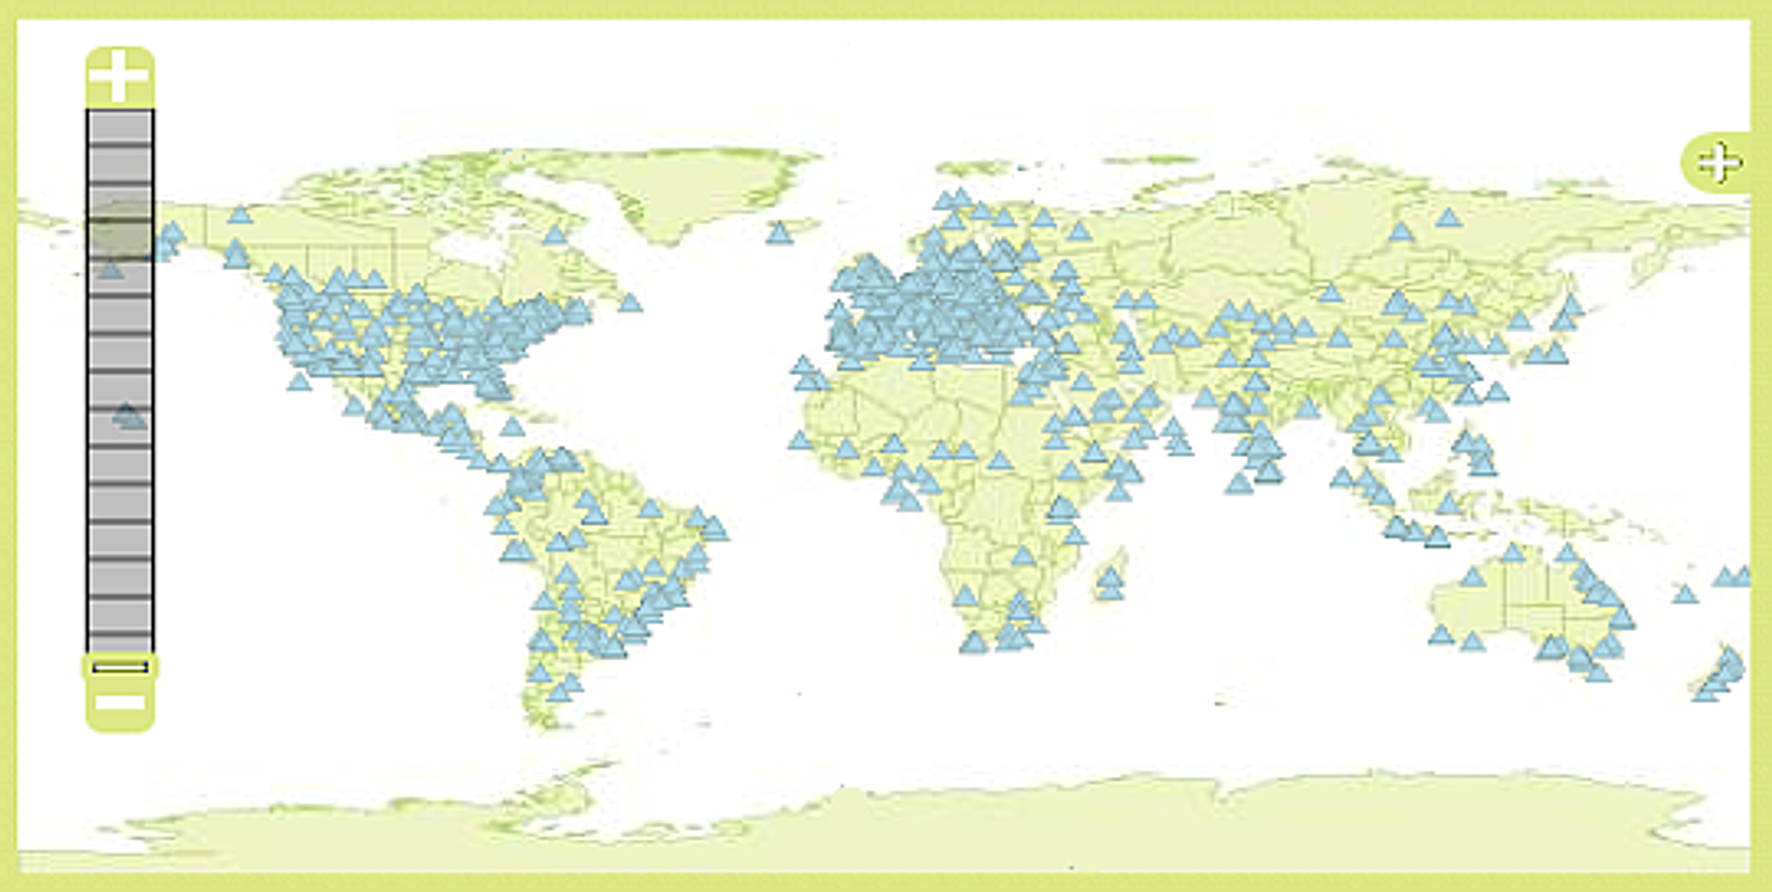
\includegraphics[clip=true]{community-map}
\end{center}
\end{figure}

There are several possibilities to get in contact with the QGIS project. 
A prefered way is is by joining the qgis-users mailing list or the QGIS Forum. 

\subsection{Functionality}

Current QGIS 1.0, released in January 2009, provides a stable API from which
you can develop custom solutions in Python or C++. Even though 1.0 is fresh,
there are a number of exciting developments underway in both the core
application and plugins. QGIS offers a growing number of common GIS
functionalities provided by core features and plugins. This includes to:

\begin{figure}[h]
   \begin{center}
   \caption{Quantum GIS 1.0.0 'Kore'}\label{fig:qgis10}\smallskip
   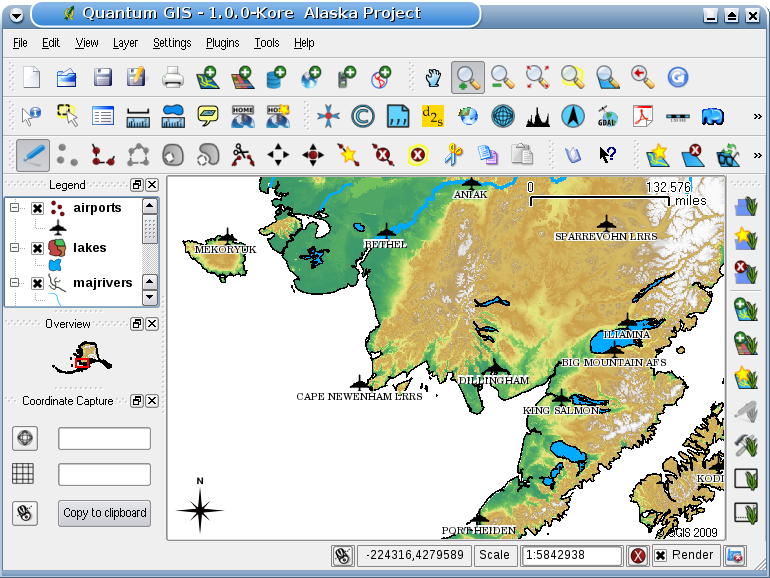
\includegraphics[clip=true, width=\textwidth]{qgis10}
\end{center}
\end{figure}

\begin{itemize}
\item view and overlay vector and raster layer in different formats and
projections without conversion to an internal or common format. Supported are
PostgreSQL/PostGIS, GDAL/OGR supported vector and raster layers such as ESRI
Shapefile, MapInfo, GML, GeoTiff or Erdas Img., GRASS locations, and
OGC-compliant WMS and WFS;
\item interactively explore data, including features such as on the fly
(OTF) projection, identify/select geometries, view, select and search
attributes, label features, change vector and raster symbology; 
\item compose print layouts adding map canvas, legend, scalebar, images and
text lables in a print composer plugin;
\item create, edit, manage and export vector layers into several formats.
Raster layer have to be imported into GRASS GIS to be edited and
exported. 
\item perform spatial geoprocessing on PostgreSQL/PostGIS and other OGR
supported vector layers including overlay, buffer, sampling, geometry and
database management. The integrated GRASS Plugin allows to include the
complete GRASS functionality of more than 300 modules.
\end{itemize}

\subsection{Plugin Architecture}

QGIS can be customized to your special needs with the help of an extensible
plugin architecture. It provides libraries that can be used to create
QGIS plugins or even new applications with C++ or Python. 

\subsection{External Python Plugin Repositories}

Most Python plugins are managed in external repositories, and can be easily
installed using the Python Plugin Installer.

\begin{figure}[h]
   \begin{center}
   \caption{QGIS Python Plugin Installer}\label{fig:python-plugin}\smallskip
   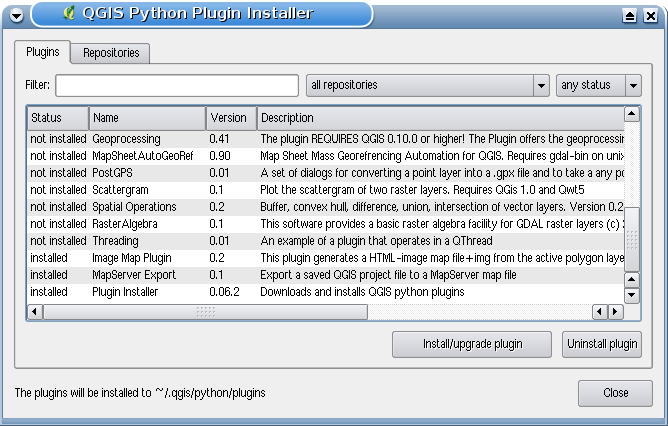
\includegraphics[clip=true, width=\textwidth]{python-plugin-installer}
\end{center}
\end{figure}


\subsection{Development}

\subsection{Perspective / Conclusion}

\minisec{Authors}

The authors of this article are QGIS Project Steering Committee Members:

Otto Dassau <dassau@nature-consult.de>  
\\Gary Sherman <sherman@mrcc.com>
\\Tim Sutton <tim@linfinity.com>
\\Marco Hugentobler <marco.hugentobler@karto.baug.ethz.ch>
\\Paolo Cavallini <cavallini@faunalia.it>

\minisec{Links}

For more information, have a look at the following website:

Quantum GIS project: http://qgis.osgeo.org
\\Open Source Geospatial Foundation: http://www.osgeo.org
 


 



